% \documentclass[handout]{beamer}
\documentclass{beamer}

\mode<presentation>
{
  \usetheme{default}
  \usefonttheme[onlymath]{serif}
  % \usetheme{Singapore}
  % \usetheme{Warsaw}
  % \usetheme{Malmoe}
  % \useinnertheme{circles}
  % \useoutertheme{infolines}
  % \useinnertheme{rounded}

  \setbeamercovered{transparent=5}
}

\usepackage[english]{babel}
\usepackage[latin1]{inputenc}
\usepackage{textpos,alltt,listings,multirow,ulem,siunitx}
\newcommand\hmmax{0}
\newcommand\bmmax{0}
\usepackage{bm}

% font definitions, try \usepackage{ae} instead of the following
% three lines if you don't like this look
\usepackage{mathptmx}
\usepackage[scaled=.90]{helvet}
% \usepackage{courier}
\usepackage[T1]{fontenc}
\usepackage{tikz}
\usetikzlibrary[shapes,shapes.arrows,arrows,shapes.misc,fit,positioning]

% \usepackage{pgfpages}
% \pgfpagesuselayout{4 on 1}[a4paper,landscape,border shrink=5mm]

\usepackage{JedMacros}

\title{Utilizing Emerging Hardware for Multiphysics Simulation Through Implicit High-Order Finite Element Methods With Tensor Product Structure}
\author{Jed Brown\inst{1}, Aron Ahmadia\inst{2}, Matt Knepley\inst{3}, Barry Smith\inst{1}}


% - Use the \inst command only if there are several affiliations.
% - Keep it simple, no one is interested in your street address.
\institute
{
  \inst{1}{Mathematics and Computer Science Division, Argonne National Laboratory} \\
  \inst{2}{King Abdullah University of Science and Technology} \\
  \inst{3}{Computation Institute, University of Chicago}
}

\date{2011-12-05}

% This is only inserted into the PDF information catalog. Can be left
% out.
\subject{Talks}


% If you have a file called "university-logo-filename.xxx", where xxx
% is a graphic format that can be processed by latex or pdflatex,
% resp., then you can add a logo as follows:

% \pgfdeclareimage[height=0.5cm]{university-logo}{university-logo-filename}
% \logo{\pgfuseimage{university-logo}}



% Delete this, if you do not want the table of contents to pop up at
% the beginning of each subsection:
% \AtBeginSubsection[]
% {
% \begin{frame}<beamer>
%   \frametitle{Outline}
%   \tableofcontents[currentsection,currentsubsection]
% \end{frame}
% }

\AtBeginSection[]
{
  \begin{frame}<beamer>
    \frametitle{Outline}
    \tableofcontents[currentsection]
  \end{frame}
}

% If you wish to uncover everything in a step-wise fashion, uncomment
% the following command:

% \beamerdefaultoverlayspecification{<+->}

\begin{document}
\lstset{language=C}
\normalem

\begin{frame}
  \titlepage
\end{frame}

\begin{frame}{The Roadmap}
  \begin{block}{Hardware trends}
    \begin{itemize}
    \item More cores (keep hearing $\bigO(1000)$ per node)
    \item Long vector registers (already 32 bytes for AVX and BG/Q)
    \item Must use SMT to hide memory latency
    \item Must use SMT for floating point performance (GPU, BG/Q)
    \item Large penalty for non-contiguous memory access
    \end{itemize}
  \end{block}
  \begin{block}{``Free flops'', but how can we use them?}
    \begin{itemize}
    \item High order methods good: better accuracy per storage
    \item High order methods bad: work unit gets larger
    \item GPU threads have very little memory, must keep work unit small
    \item Need library composability, keep user contribution embarrassingly parallel
    \end{itemize}
  \end{block}
\end{frame}

\begin{frame}{How to program this beast?}
  \begin{itemize}
  \item Decouple physics from discretization
    \begin{itemize*}
    \item Expose small, embarrassingly parallel operations to user
    \item Library schedules user threads for reuse between kernels
    \item User provides physics in kernels run at each quadrature point
    \item Continuous weak form: find $u \in \VV_D$
      \[ v^T F(u) \sim \int_\Omega v \cdot {\color{green!70!black} f_0(u,\nabla u)}
      + \nabla v \tcolon {\color{green!70!black} f_1(u,\nabla u)} = 0, \qquad \forall v \in \VV_0 \]
    \item Similar form at faces, but may involve Riemann solve
    \end{itemize*}
  \item Library manages reductions
    \begin{itemize*}
    \item Interpolation and differentiation on elements
    \item Exploit tensor product structure to keep working set small
    \item Assembly into solution/residual vector (sum over elements)
    \end{itemize*}
  \end{itemize}
\end{frame}

\begin{frame}{Nodal $hp$-version finite element methods}
  \begin{columns}
    \begin{column}{0.4\textwidth}
      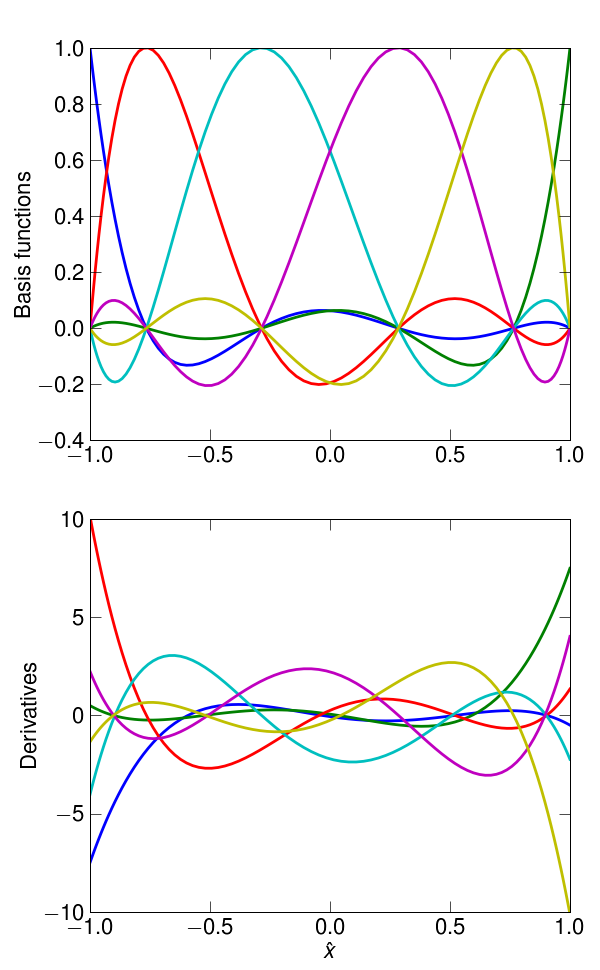
\includegraphics[width=\textwidth]{figures/lgl}
    \end{column}
    \begin{column}{0.6\textwidth}
      \begin{block}{1D reference element}
        \begin{itemize}
        \item Lagrange interpolants on Legendre-Gauss-Lobatto points
        \item Quadrature $\hat R$, weights $\hat W$
        \item Evaluation: $\hat B, \hat D$
        \end{itemize}
      \end{block}
      \vspace{-1em}
      \begin{block}{3D reference element}
      \vspace{-1em}
        \begin{align*}\label{eq:tprod}
          \begin{split}
            % \hat{\bm R} &= \hat R \otimes \hat R \otimes \hat R \\
            \hat{\bm W} &= \hat W \otimes \hat W \otimes \hat W \\
            \hat{\bm B} &= \alert<2>{\hat B \otimes \hat B \otimes \hat B} \\
          \end{split} &
          \begin{split}
            \hat{\bm D}_0 &= \alert<2>{\hat D \otimes \hat B \otimes \hat B} \\
            \hat{\bm D}_1 &= \alert<2>{\hat B \otimes \hat D \otimes \hat B} \\
            \hat{\bm D}_2 &= \alert<2>{\hat B \otimes \hat B \otimes \hat D} \\
          \end{split}
        \end{align*}
        \vspace{-1em}
        \begin{block}<2>{\alert{These tensor product operations \\ 
              are very efficient, 70\% of peak flop/s}}
        \end{block}
      \end{block}
    \end{column}
  \end{columns}
\end{frame}

\begin{frame}{Operations on physical elements}
  \begin{block}{Mapping to physical space}
    \vspace{-2em}
    \begin{gather*}
      x^e : \hat K \to K^e,\quad J^e_{ij} = \partial x_i^e/\partial \hat x_j, \quad (J^e)^{-1} = \partial \hat x/\partial x^e \\
    \end{gather*}
  \vspace{-2em}
  \end{block}
  \vspace{-2em}
  \begin{block}{Element operations in physical space}
  \vspace{-2em}
    \begin{align*}
      \bm B^e &= \hat{\bm B} \qquad \qquad \qquad \bm W^e = \hat{\bm W} \Lambda(\abs{J^e(\bm r)}) \\
      \bm D^e_i &= \Lambda\left(\frac{\partial \hat x_0}{\partial x_i}\right) \hat{\bm D}_0
      + \Lambda\left(\frac{\partial \hat x_1}{\partial x_i}\right) \hat{\bm D}_1
      + \Lambda\left(\frac{\partial \hat x_2}{\partial x_i}\right) \hat{\bm D}_2 \\
      (\bm D^e_i)^T &= \hat{\bm D}_0^T \Lambda\left(\frac{\partial \hat x_0}{\partial x_i}\right)
      + \hat{\bm D}_1^T \Lambda\left(\frac{\partial \hat x_1}{\partial x_i}\right)
      + \hat{\bm D}_2^T \Lambda\left(\frac{\partial \hat x_2}{\partial x_i}\right)
    \end{align*}
  \end{block}
  \vspace{-2em}
  \begin{block}{Global problem is defined by assembly}
  \vspace{-2em}
  \begin{equation*}
    F(u) =
    \sum_e \EE_e^T \Big[ (\bm B^e)^T \bm W^e \Lambda({\color{green!70!black} f_0(u^e,\nabla u^e)})
    + \sum_{i=0}^d(\bm D_i^e)^T \bm W^e \Lambda({\color{green!70!black} f_{1,i}(u^e,\nabla u^e)}) \Big] = \bm 0
  \end{equation*}
  where $u^e = \bm B^e \EE^e u$ and $\nabla u^e = \{\bm D_i^e \EE^e u\}_{i=0}^2$
  \end{block}
\end{frame}

\begin{frame}[shrink=5]{Representation of Jacobians, Automation}
  \begin{itemize}
  \item For unassembled representations, decomposition, and assembly
  \item Continuous weak form: find $u$
    \[ v^T F(u) \sim \int_\Omega v \cdot {\color{green!70!black} f_0(u,\nabla u)}
    + \nabla v \tcolon {\color{green!70!black} f_1(u,\nabla u)} = 0, \qquad \forall v \in \VV_0 \]
  \item Weak form of the Jacobian $J(u)$: find $w$
    \begin{gather*}
      v^T J(u) w \sim \int_\Omega \begin{bmatrix} v^T & \nabla v^T \end{bmatrix}
      {\color{blue} \begin{bmatrix} f_{0,0} & f_{0,1} \\ f_{1,0} & f_{1,1} \end{bmatrix}}
      \begin{bmatrix} w \\ \nabla w \end{bmatrix} \\
      {\color{blue} [f_{i,j}] = \begin{bmatrix} \dfrac{\partial f_0}{\partial u} & \dfrac{\partial f_0}{\partial \nabla u} \\[1em]
          \dfrac{\partial f_1}{\partial u} & \dfrac{\partial f_1}{\partial \nabla u} \end{bmatrix} (u,\nabla u) }
    \end{gather*}
  \item Terms in ${\color{blue} [f_{i,j}]}$ easy to compute symbolically, AD more scalable.
  \item Nonlinear terms ${\color{green!70!black}f_0,f_1}$ usually have the most expensive nonlinearities in the computation of scalars
    \begin{itemize}
    \item Equations of state, effective viscosity
    \item Compute gradient with reverse-mode, store at quadrature points.
    \item Perturb scalars, then use forward-mode to complete the Jacobian.
    \item Flip for action of the adjoint.
    \end{itemize}
  \end{itemize}
\end{frame}

\newcommand\smallterm[1]{{\color{gray} #1}}
\begin{frame}{Conservative (non-Boussinesq) two-phase ice flow}
  Find momentum density $\rho\uu$, pressure $p$, and total energy density $E$:
  \begin{gather*}
    (\rho\uu)_t + \div (\smallterm{\rho\uu\otimes\uu} - \eta D\uu_i + p\bm 1) - \rho \bm g = 0 \\
    \rho_t + \div \rho\uu = 0 \\
    E_t + \div \big((E+p)\uu - k_T\nabla T - k_\omega\nabla\omega \big) - \eta D\uu_i\tcolon D\uu_i - \smallterm{\rho\uu\cdot\bm g} = 0
  \end{gather*}
\begin{itemize}
\item Solve for density $\rho$, ice velocity $\uu_i$, temperature $T$, and melt fraction $\omega$ using constitutive relations.
  \begin{itemize}
  \item Simplified constitutive relations can be solved explicitly.
  \item Temperature, moisture, and strain-rate dependent rheology $\eta$.
  \item High order FEM, typically $Q_3$ momentum \& energy, SUPG (yuck).
  \end{itemize}
\item DAEs solved implicitly after semidiscretizing in space.
\item Preconditioning using nested fieldsplit
\end{itemize}
\end{frame}

\begin{frame}[fragile,shrink=5]{Traversal code}
  \begin{itemize*}
  \item CPU traversal computes coefficients of test functions, \url{https://github.com/jedbrown/dohp/}
  \begin{ccode}
  while (IteratorHasPatch(iter)) {
    IteratorGetPatchApplied(iter,&Q,&jw,
        &x,&dx,NULL,NULL,
        &u,&du,&u_,&du_, &p,&dp,&p_,NULL, &e,&de,&e_,&de_);
    IteratorGetStash(iter,NULL,&stash);
    for (dInt i=0; i<Q; i++) {
      PointwiseFunction(context,x[i],dx[i],jw[i],
          u[i],du[i],p[i],dp[i],e[i],de[i],
          &stash[i], u_[i],du_[i],p_[i],e_[i],de_[i]);
    }
    IteratorCommitPatchApplied(iter,INSERT_VALUES, NULL,NULL,
                               u_,du_, p_,NULL, e_,de_);
    IteratorNextPatch(iter);
  }
  \end{ccode}
  \item GPU version calls \cfunc|PointwiseFunction| directly.
  \item Unassembled Jacobian application reuses \cverb|stash|
    \begin{ccode}
  PointwiseJacobian(context,&stash[i],dx[i],jw[i],
                    u[i],du[i],p[i],dp[i],e[i],de[i],
                    u_[i],du_[i],p_[i],e_[i],de_[i]);
    \end{ccode}
  \end{itemize*}
\end{frame}

\begin{frame}
  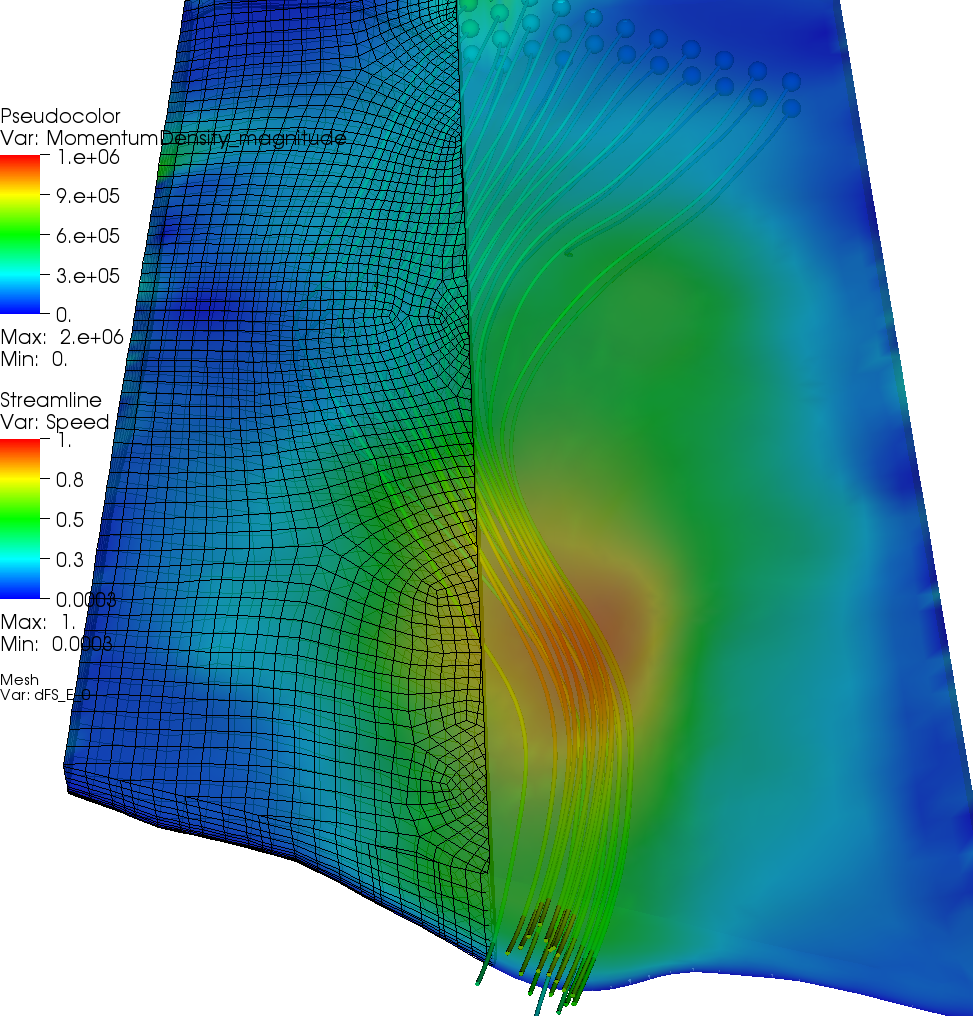
\includegraphics[width=\textwidth]{figures/VHT/TopViewStreamline}
\end{frame}
\begin{frame}
  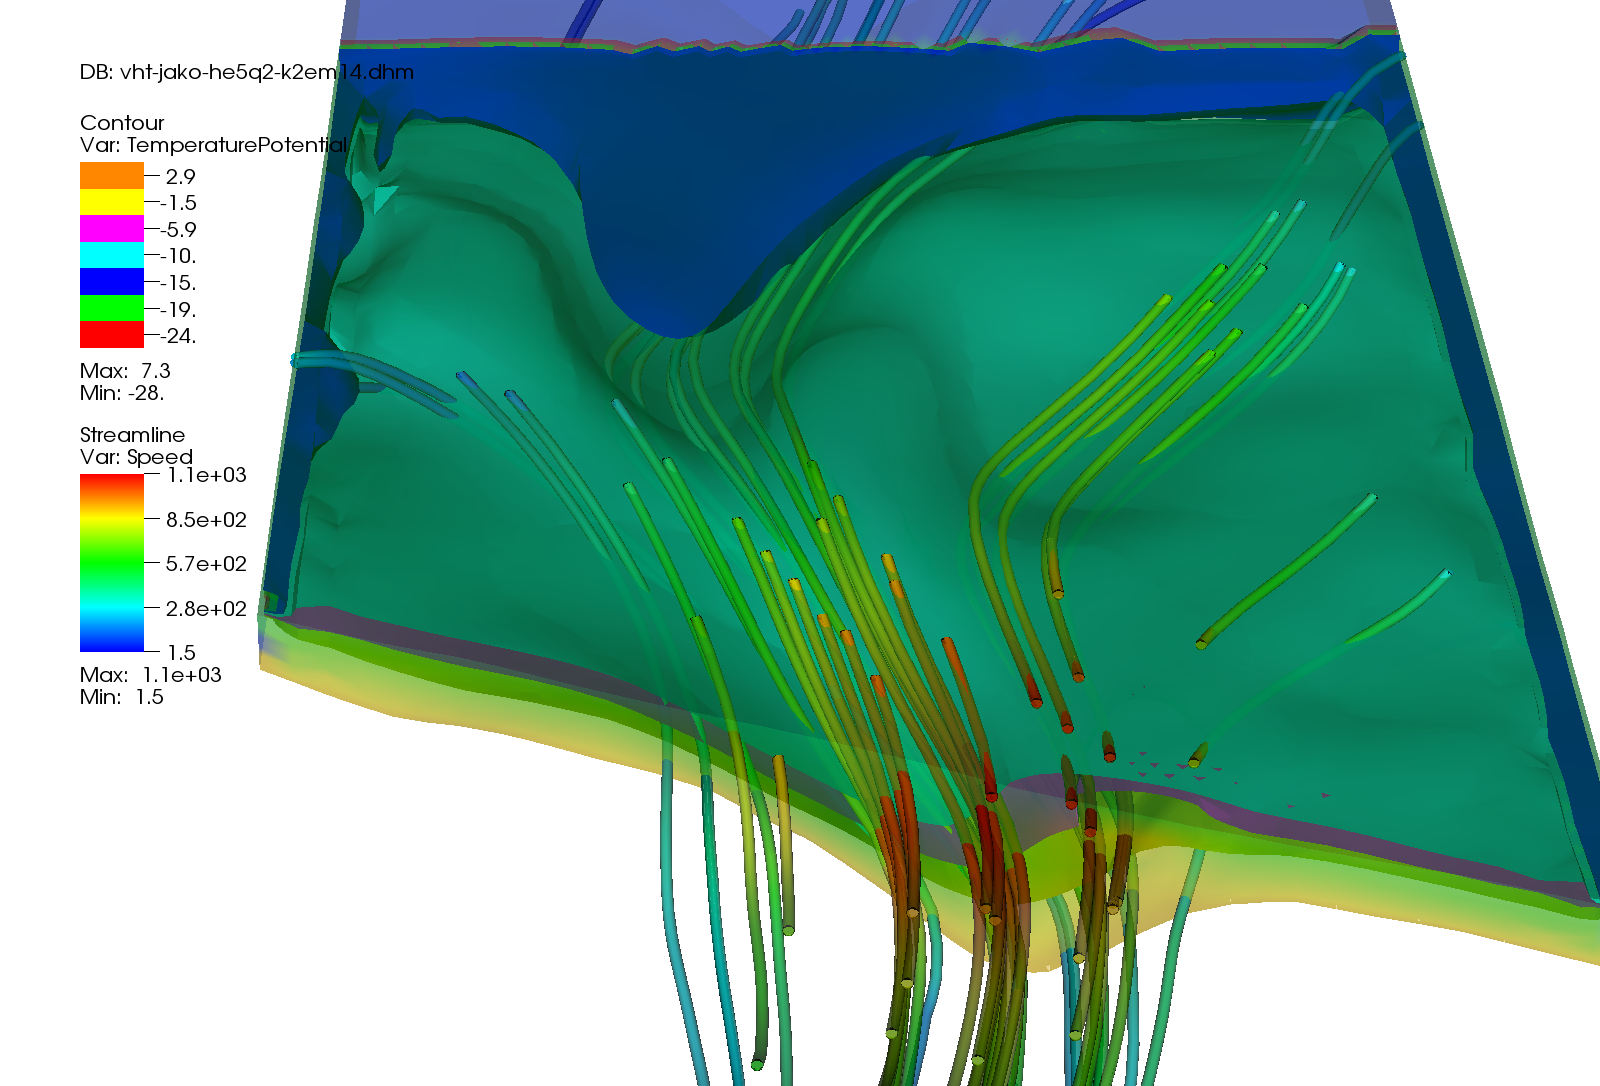
\includegraphics[width=\textwidth]{figures/VHT/VHTJakoContourStream}
\end{frame}

\begin{frame}[shrink=5]{Performance of assembled versus unassembled}
  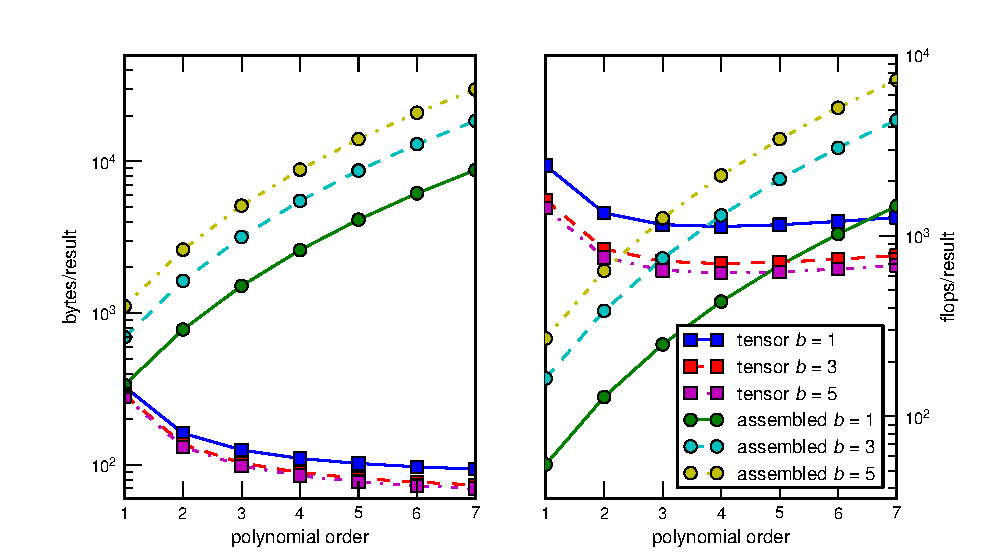
\includegraphics[width=\textwidth]{figures/TensorVsAssembly} \\
  \begin{itemize}
  \item High order Jacobian stored unassembled using coefficients at quadrature points, can use local AD
  \item Choose approximation order at run-time, independent for each field
  \item Precondition high order using assembled lowest order method
  \item Implementation $> 70\%$ of FPU peak, SpMV bandwidth wall $< 4\%$
  \end{itemize}
\end{frame}


\begin{frame}{Memory Bandwidth}
  \begin{tabular}{lc}
    \toprule
    Operation                         & Arithmetic Intensity (flop/s per byte) \\
    \midrule
    Sparse matrix-vector product      & 1/6                  \\
    Dense matrix-vector product       & 1/4                  \\
    Unassembled matrix-vector product & $\approx 8$          \\
    High-order residual evaluation    & $> 5$                \\
    \bottomrule
  \end{tabular}
  \bigskip
  \begin{tabular}{lrrr}
    \toprule
    Processor           & BW (GB/s) & Peak (GF/s) & Balanced AI (F/s/B) \\
    \midrule
    Sandy Bridge 6-core & 21*       & 150         & 7.2                 \\
    Magny Cours 16-core & 42*       & 281         & 6.7                 \\
    Blue Gene/Q node    & 43        & 205         & 4.8                 \\
    GeForce 9400M       & 21        & 54          & 2.6                 \\
    GTX 285             & 159       & 1062        & 6.8                 \\
    Tesla M2050         & 144       & 1030        & 7.1                 \\
    \bottomrule
  \end{tabular}
\end{frame}

\begin{frame}{Outlook}
  \begin{itemize}
  \item Sparse matrix assembly (for preconditioning) not shown
    \begin{itemize}
    \item $> 100$ GF/s for lowest order Stokes (Matt Knepley)
    \item common physics code with CPU implementation
    \item Dohp CPU version faster than libMesh and Deal.II for $Q_1$
    \item $Q_1$ assembly embedded in higher order is 8\% slower than hand-rolled
    \end{itemize}
  \item Can't wait for OpenCL to implement indirect function calls
  \item Symbolic differentiation too slow, tired of hand-differentiation
  \item I want source-transformation AD with indirect function calls
  \item Find correct amount of reuse between face and cell integration
  \item Riemann solves harder to vectorize
  \item Finer grained parallelism in GPU tensor product kernels
  \item Hide dispatch to pointwise kernels inside library
    \begin{itemize}
    \item Easy, but scary. Library/framework becomes \alert{\bf F}ramework.
    \end{itemize}
  \end{itemize}
\end{frame}

\end{document}
